\chapter{Whole System Emulation}

Virtualization is the process of abstracting the hardware components of a system in order to make them available to software in a virtual form.

There are different reasons behind the choice to virtualize an environment and many different methods to do it correctly according to the different needs. For example on a shared server one might want to allocate a virtual machine to each user, in order to have maximum efficiency and fully take advantage of the underlying hardware all the virtual machines should reside to the lowest possible hardware level. Meaning that the more they operate directly on the hardware the less is the overhead introduced.

Another possible use case is a developer that might want to cross compile applications on his pc. One way to achieve this is to have multiple virtual machines, each with a different operating system, and then run a compiler on each VM. It is clear that this is a different task which has different requirements compared to the previous one.

Lastly the creation of virtual environments allows for a better management and security of the environment, as a matter of fact virtual machines acts as physically separated individual computers whose resources can easily be managed and machines as well as users can be segregated. As virtual machines run on virtual hardware and the resources are segregated there is little to no interaction between different virtual machines on the same physical hardware. This is particularly interesting as for example in the event of a security incident the network adapter can be removed from the affected virtual machine and it can also be reverted to a pristine state using a snapshot. 

The Operating System on top of which the virtualization software runs is called Host OS while the Operating System that run inside each virtual machine is called Guest OS. 

\section{A bit of background: the Hypervisor}

At the core of the virtualization process there is the Hypervisor. The hypervisor is a piece of code whose definition blends with the one of operating system. Hypervisors are also commonly referred as Virtual Machine Managers (VMM) as they take care of all the tasks related to the management of resources and integration between physical and virtual machine effectively creating an interface between the two.

Virtualization requirements have been defined in \cite{virtreq} and proposes a set of properties that Virtual Machine Monitor should have:

\begin{itemize}
    \item \textbf{Equivalence / Fidelity:} A program running under the VMM should exhibit a behavior essentially identical to that demonstrated when running on an equivalent machine directly.
    \item \textbf{Resource control / Safety:} The VMM must be in complete control of the virtualized resources.
    \item \textbf{Efficiency / Performance:} A statistically dominant fraction of machine instructions must be executed without VMM intervention.
\end{itemize}

Although in the years such properties have been revised and nowadays for a VMM to be satisfying it is sufficient that it verifies the first two. 

As described in\cite{os} there are 3 different types of hypervisors: \textbf{Type 0}, \textbf{Type 1} and \textbf{Type 2}. 

Modern processors have virtualization support built in the hardware meaning that the processor offers an additional layer on top of which the VMM can operate. On top of this it is possible to have a hardware hypervisor, often referred as \textbf{Type 0}, which is a piece of code running directly on the hardware and taking care of allocating the right amount of resources and handle hardware-software interactions. This method is really close to running a proper operating system directly on the hardware as each virtual machine created by a\textbf{Type 0} Hypervisor effective runs, in turn, on the physical CPU. For this reason each VM created in this way can be a different kind of VMM itself.

In addition to this all modern CPU implements a form of Hardware Assisted Virtualization, called VT-x for Intel and AMD-V for AMD. Hardware virtualization allows for better performance and easy maintaining of the virtualization software by expanding the CPU instruction set with some dedicated instructions. 

A graphical representation of the differences between the other two types of hypervisors can be found in Figure \ref{fig:hip}.

\begin{figure}[htp]
\centering
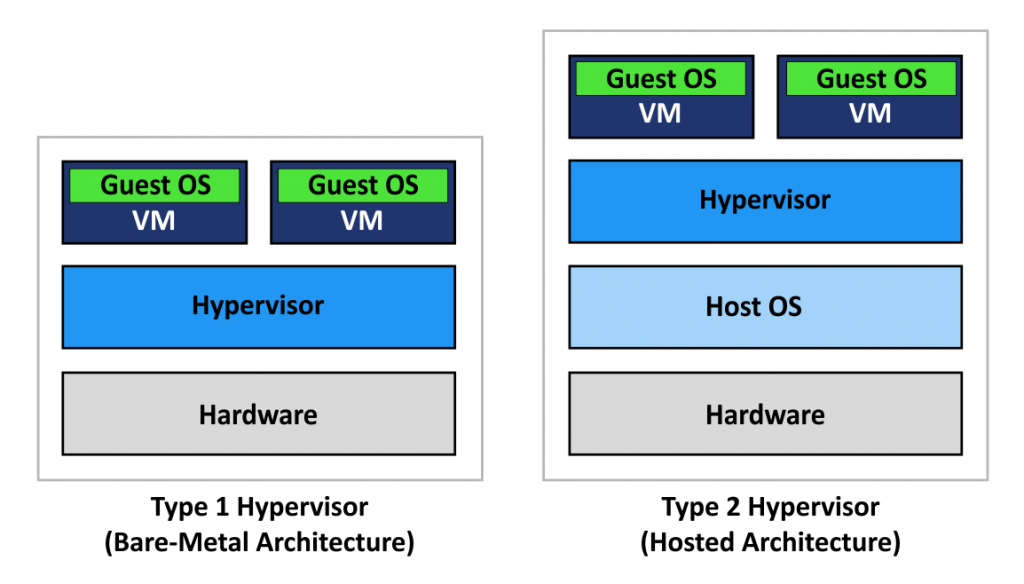
\includegraphics[width=\linewidth]{images/hip.png}
\caption{Hypervisors types \newline \url{https://netseedblog.com/security/virtualization-forensics-part-1/}}
\label{fig:hip}
\end{figure}



\subsection{Type 1 or bare metal}

The \textbf{Type 1} or "Bare Metal" hypervisor is a a sort of specialized operating system that is dedicated only to the management of virtual machines. This is very commonly found on servers, particularly in data-centers where it is necessary to have high efficiency on single servers. For this reason VMs that run on this type of hypervisor can achieve very high performances as a matter of fact, similarly to \textbf{Type 0}, they allow guest VMs to run directly on the hardware. Examples of this kind of hypervisor are VMWare ESX and Xen.

Moreover even non specialized operating systems such as Linux, Windows and MacOS have support for virtualization and can act as \textbf{Level 1} hypervisors. As they are not dedicated VMMs they provide fewer control and customization of the virtualized environment and they treat the virtual machine like every other process. However, virtual machines run on this kind of hypervisor are still efficient as they will be granted direct access to system resources. 

\subsection{Level2 or hosted}

The Level 2 hypervisor is a dedicated piece of software which provides another level of abstraction as it runs on top of an existing operating system. Virtual Machines running on top of this hypervisor will not have access to the real physical hardware and instead they will access an emulated and standardized architecture. In this way the user can have more control on the resources and the virtualized environment, trading in some performances. 

It must be noted that nowadays this two level of hypervisors can, sometimes, blending together. For example Linux KVM (Kernel Based Virtual Machine) is a kernel module available in modern Linux distributions that transforms the operating system into a \textbf{Level 1} hypervisor while still retaining all the other OS functionalities.

\section{Emulation}
\todo{Review the below points}
Virtualization brings some benefits mainly in terms of:
\begin{itemize}
    \item \textbf{Efficiency} as multiple virtual machines can be run on a single physical machine optimizing the usage of resources.
    \item \textbf{Cost reduction} derived directly form the above one, by more efficiently utilizing a single machine it is possible to "do more with less".
    \item \textbf{Compatibility} as different Operating Systems can run on a single host OS this allows to run, compile or test different applications on top of a single environment almost closing the gap between the various architectures.
    \item \textbf{Easier testing} as different architectures can be emulated on top of a single machine this allows to develop programs for different architectures bypassing some unnecessary steps, for example an application for a phone can be complied and tested on a normal laptop and then pushed to the phone only when the final version is ready.
    \item \textbf{Security} perhaps the most important fact, as virtual machines are all isolated between them and between the guest os they can be managed in a better way. Moreover the ability to take snapshot of a certain state and then revert the machine back to it makes it more resilient to attacks, avoids potential data loss and makes it more resilient to software faults. 
\end{itemize}

As discussed above there are different approaches that can be taken to virtualize an environment. One of the most interesting techniques is \textbf{Emulation}. 

Emulation takes virtualization even further as, instead of utilizing the same hardware (virtual or physical) that resides on the computer, fully emulates the CPU. This means that the CPU is not an hardware component anymore but, instead, all its functionalities are translated in code. 
In this way the virtual cpu acts as a glue-layer between the two architectures by translating emulated instructions into native ones. This is particularly interesting as it allows the computer to run programs compiled for completely different CPUs. 

\section{Virtual Machines}

With the term Virtual Machine we usually refer to \textbf{Type 2} hypervisors.

There are available different solutions to create virtual machines, both open source and commercial ones. Between the open source solutions \textbf{Virtual Box} and \textbf{QEMU} are the most common while on the commercial side \textbf{VMWare} and \textbf{Paralles} are the main players. 

There are many things that must be coordinated under the hood in order to successfully trick the Guest OS into believing that it is running on a physical machine and has dedicated resources. Some peculiar aspects are memory management and CPU scheduling.

On the memory management side there is a high pressure on the real memory which will be used by the Host OS, Guest OS and by the VMM itself. There is therefore a need for an efficient management of the RAM:

\textit{"Before memory optimization can occur, the VMM must establish how much real memory each guest should use. To do that, the VMM first evaluates each guest’s maximum memory size. General-purpose operating systems do not expect the amount of memory in the system to change, so VMMs must maintain the illusion that the guest has that amount of memory. Next, the VMM computes a target real-memory allocation for each guest based on the configured memory for that guest and other factors, such as over commitment and system load"}\cite{os}

The physical CPU will be under stress as well as it will be shared between Guest OS, Host OS and VMM. This last software has access to the real hardware and can therefore steal CPU cycles from the Guest OSs to schedule its tasks for VM Management.
\textit{"More difficult is the case of over commitment, in which the guests are configured for more CPUs than exist in the system. Here, a VMM can use standard scheduling algorithms to make progress on each thread but can also add a fairness aspect to those algorithms"}\cite{os}

I/O is another interesting aspect of the virtualization that must be taken into account, a VMM must create proper virtual devices such as Network Bridges in order to allow each machine to connect to the network. There are moreover devices such as webcams or USB storage which cannot be accessed concurrently therefore there is no alternative if not to allow a single machine at the time to use them.

\subsection{QEMU}

QEMU is a powerful open source virtualization software which can be operated in two modes: 

\textbf{User-Mode emulation} which allows qemu to run programs compiled for a CPU on another CPU.

\textbf{Full System Emulation} where QEMU acts as a proper \textbf{Type 2} hypervisor allowing to run proper virtual machines. In this operating mode QEMU can also take advantage of KVM to run virtual machines at Linux Kernel level and achevie near native performances. 

QEMU is highly modular and can easily be expanded to add more functionalities. Moreover its structure allows a great control over the virtual machine architecture allowing to tap into each single internal component of the machine such as CPU registers and ram. Due to its nature QEMU has been used in many different projects however it still lacks some of the feature of more modern and user friendly virtualization solutions such as Virtual Box or VMWare.

Moreover QEMU supports a large set of different architectures which makes it useful not only to create virtual machines but also for low level OS development.
\todo{Qemu monitor, qemu intermediate language}

\subsection{Java Virtual Machine: an uncommon one}

When thinking about virtual machines one often thinks about ways to virtualize an operating system. Virtualization is however used also in programming languages as a matter of fact the Java language implements its own virtual machine. Each java class is compiled in an architecture neutral bytecode output which will then be run inside the JVM. This VM will then take care of translating java opcodes into the real ones. In this way it is sufficient to ship different JVMs for the different architectures and each program that is written in java will run on top of it.  
\section{Other possible approaches}
\todo{has docker ever been used for malware analysis? \url{https://www.reddit.com/r/docker/comments/eakd50/help_can_i_safely_run_malware_inside_a_container/}
\url{https://ieeexplore.ieee.org/abstract/document/9042158}}

% take a look https://www.blackhat.com/docs/us-14/materials/us-14-Kruegel-Full-System-Emulation-Achieving-Successful-Automated-Dynamic-Analysis-Of-Evasive-Malware-WP.pdf